\documentclass[12pt]{article}
\usepackage{array}
\usepackage{amsmath}
\usepackage{amssymb}
\usepackage{algorithm}
\usepackage{algorithmic}
\usepackage{caption}
\usepackage{fontspec}
\usepackage{graphicx}
\usepackage{indentfirst}
\usepackage{minted}
\usepackage{mathtools}
\usepackage{pifont}
\usepackage{setspace}
\usepackage{subfigure}
\usepackage{tikz}
\usepackage{url}
\usepackage{xcolor}
\usepackage{xeCJK}

\usepackage[colorlinks=true]{hyperref}
\usepackage[margin=0.55in]{geometry}

% background color for minted
\definecolor{bg}{rgb}{0.95,0.95,0.95}

% CJK font
\setCJKmainfont{Source Han Serif CN}

% indent value
\setlength{\parindent}{2em}

% line spacing
\linespread{1.2}

% C++ styled text
\newcommand{\CC}{C\nolinebreak\hspace{-.05em}\raisebox{.4ex}{\tiny\bf +}%
\nolinebreak\hspace{-.10em}\raisebox{.4ex}{\tiny\bf +}}

\title{{C++}11: The Rule of the Big Five}
\author{Yiteng Zhang}

\begin{document}
\maketitle

\indent{}这大体上是一篇译文,原文来自 Feabhas 上的同名文章。通过阅读这篇文章来复习和加深理解 {\CC}11 的五之法则
(Big-Five)。这个议题虽然非常基础,但在工程上还是比较有意义的。另外,这篇文章还涉及到许多使用{\CC}11 时的常用
知识,我在其基础上添加了一些扩展内容。

\section*{资源管理(Resource Management)}
\indent{}在 C 语言中,对象的动态创建和析构总是像怪物一般难以对付,令人头痛不已。程序员需要手动地控制对象
的内存分配,处理对象的初始化过程,保证对象在使用后会被安全地清理,并将其内存归还给堆。因为很多 C 程序员
未被那些潜在的问题教导过,C 语言常被看作不安全,容易内存泄露的语言。

\indent{}{\CC}通过引入所谓 RAII(Resource Acquisition Is Initialisation)/ RRID(Resource Release Is Destruction)
的惯用法极大地改善了各种问题。这个惯用法利用了一个事实:每次对象被创建时,一个构造函数会被调用;当对象离开
作用域时,一个析构函数会被调用。这样,构造函数与析构函数构成一对儿,用于创建/销毁一个对象,该对象被用于管理另一个对象。
对象被创建时,它会自动地为其所管理的对象分配空间并进行初始化。当对象离开作用域时,被其管理的对象会被自动地清理。
这种机制即是资源管理。一个资源可以是需要被动态创建与销毁的任何对象,可以是文件、sockets、互斥量等。

\indent{}资源管理使得我们不必为被管理对象的生命期而忧虑,潜在地消除了内存泄露和一些其他相关的问题。然而,RAII/RRID 并非没有
代价。引入一个“管理者”对象可能会导致一些潜在的问题,特别是当“管理者”在系统中传递的时候。拷贝一个“管理者”对象是首要的
议题,著名的三之法则(The Rule of The Big Three)强调了这一议题。自{\CC}11后,移动语义(Move Semantic)被加入到语言
之中,这又为议题增添了一些复杂性,因而出现了五之法则。五之法则指出,如果你不得不为下述五个函数之一提供实现,你就需要
为所有的这些函数提供相应的策略:
\begin{enumerate}
    \item 析构函数(The Destructor)
    \item 赋值运算符(The Assignment Operator)
    \item 拷贝构造函数(The Copy Constructor)
    \item 移动构造函数(The Move Constructor)
    \item 移动赋值运算符(The Move Assignment operator)
\end{enumerate}

\indent{}接下来,我们将分别对上述五个函数进行讨论,考虑在设计类的时候可能存在的一些问题。在讨论中,
我们会使用\texttt{SocketManager}类与\texttt{Socket}类作为例子。其中,\texttt{SocketManager}类管理着
\texttt{Socket}类的生命期,即\texttt{SocketManager}为\texttt{Socket}类对象的生命期负责。

\section{析构函数}
\noindent{}我们来看一看这两个类的结构:

\begin{figure}[h]
\centering
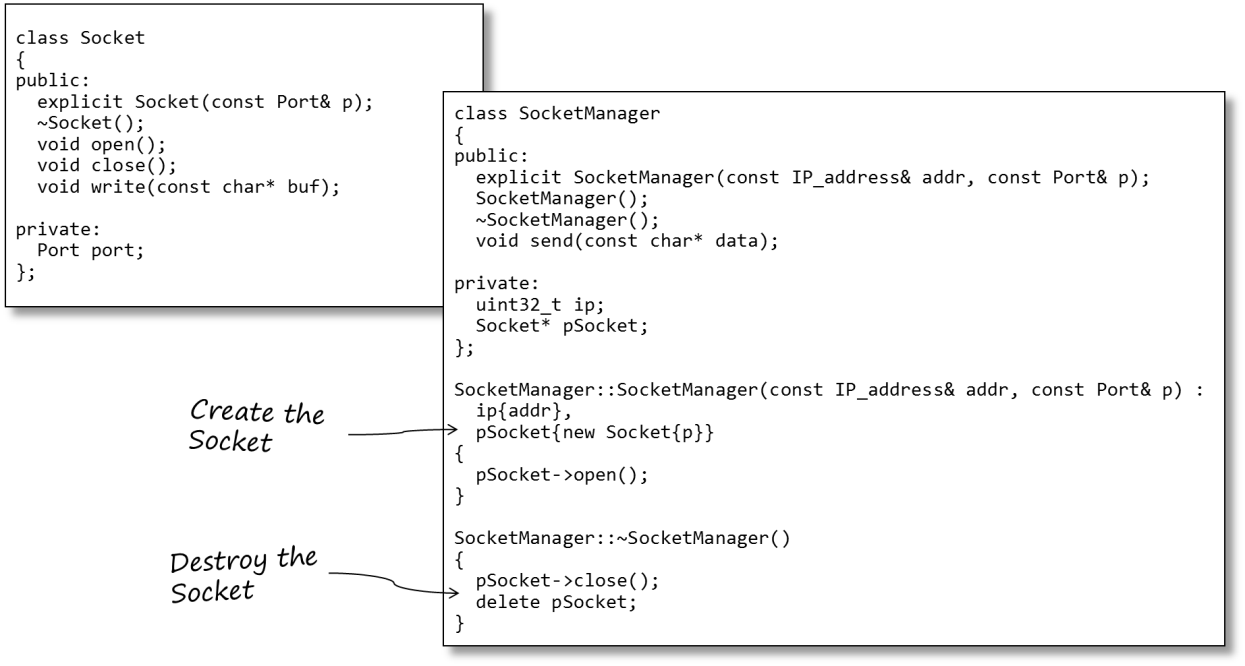
\includegraphics[width=16cm]{./imgs/image.Y7UIS0.png}
\end{figure}

\indent{}值得一提的是,在设计“管理者”类时,有两个小点需要注意一下:首先,如果你打算将你的资源管理类实现为多态基类,
那么最好让它的析构函数是虚函数。这样,我们可以保证其任何派生类的析构函数(如果被定义的话)会被正确调用。
另外,必须确保\texttt{new}和\texttt{delete}是成对而匹配的,如果资源通过\texttt{new}被分配,那么就需要对其有相应
的\texttt{delete}。下面是\texttt{SocketManager}对象的内存布局:

\begin{figure}[h]
\centering
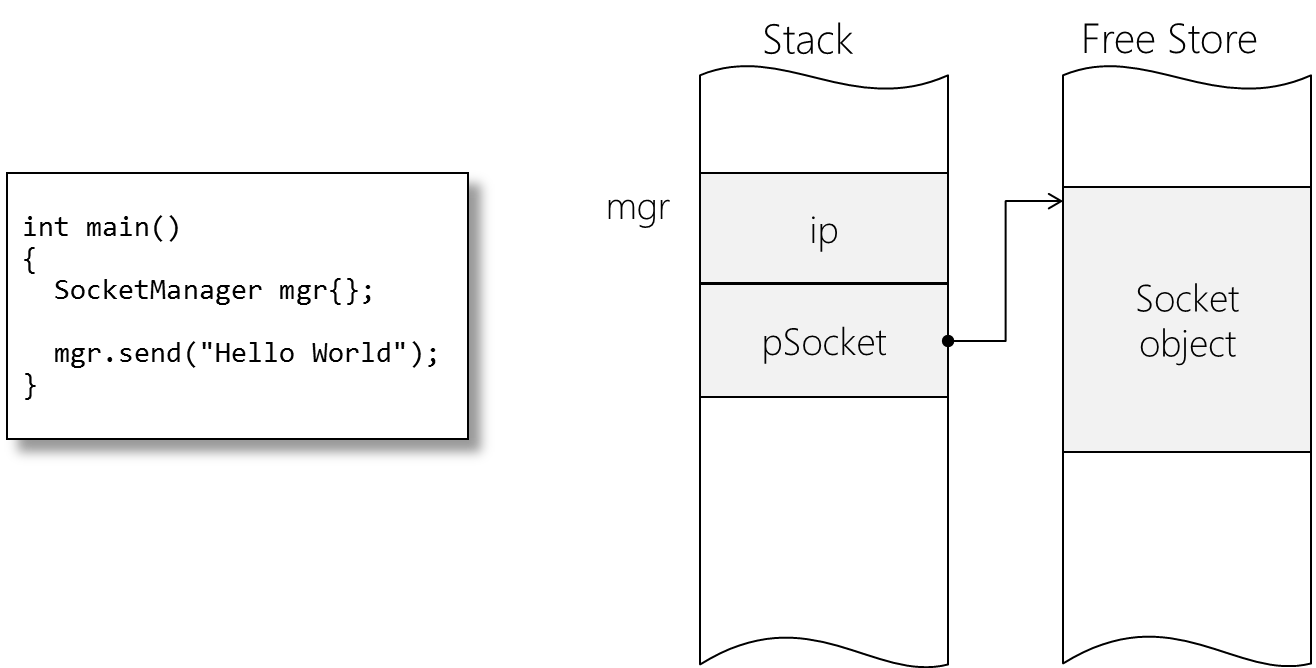
\includegraphics[width=12cm]{./imgs/image.0V3MS0.png}
\end{figure}

\indent{}当对象\texttt{mgr}离开作用域时,它的析构函数会被自动调用,进而执行\texttt{delete pSocket},那么,在
\texttt{Socket}的内存被释放之前,会调用\texttt{Socket}的析构函数。

\section{赋值运算符}
\indent{}如果你没有为类提供赋值运算符,编译器会创建一个默认的赋值运算符。默认的赋值运算符是一个
member-wise copy function,每个数据成员会一个接一个地被拷贝。现在,让我们思考一种情形,如果我们
要将一个管理者对象赋值给另一个管理者对象,会发生什么?

\begin{figure}[h]
\centering
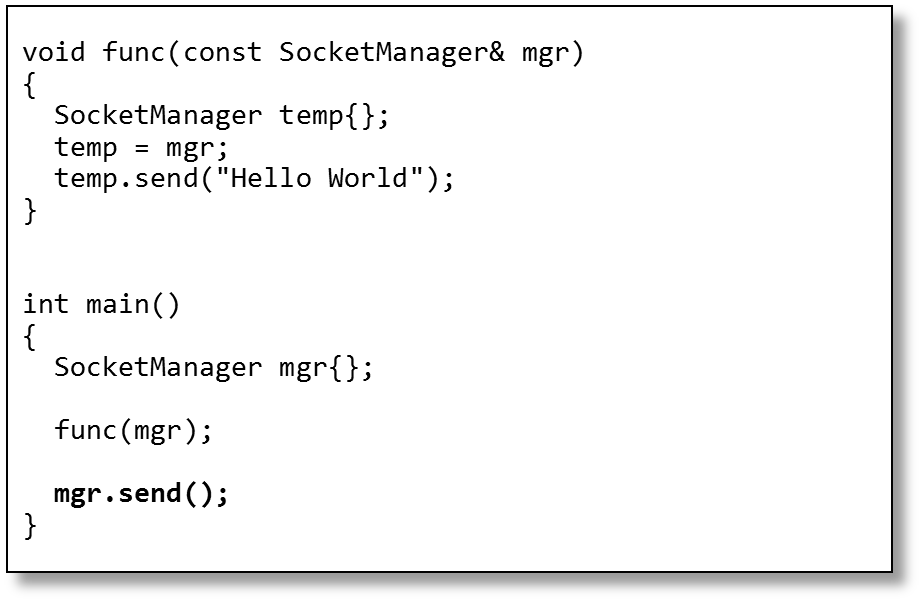
\includegraphics[width=10cm]{./imgs/image.4Y1GS0.png}
\end{figure}

\indent{}上图的例子乍一看似乎没有什么问题。然而,仔细观察后会发现,在\texttt{func()}中创建的临时的
\texttt{SocketManager}对象确实会带来问题。因为默认的赋值运算符会做 member-wise copy,那么对象\texttt{mgr}中的
指向\texttt{Socket}类的指针会被拷贝到对象\texttt{temp}中。当对象\texttt{temp}离开作用域时,会去\texttt{delete}
这个指针(因为 RRID)。由于\texttt{mgr}对象也保有这个指针,当\texttt{mgr}离开作用域时,同样会去\texttt{delete}
这个指针,但是这个指针指向的那块内存已经在\texttt{temp}离开作用域时被释放过了!实际上,在调用过\texttt{func()}
之后,如果再使用\texttt{mgr}去执行借由\texttt{pSocket}进行的任何工作,其行为将是不正常的。

\begin{figure}[h]
\centering
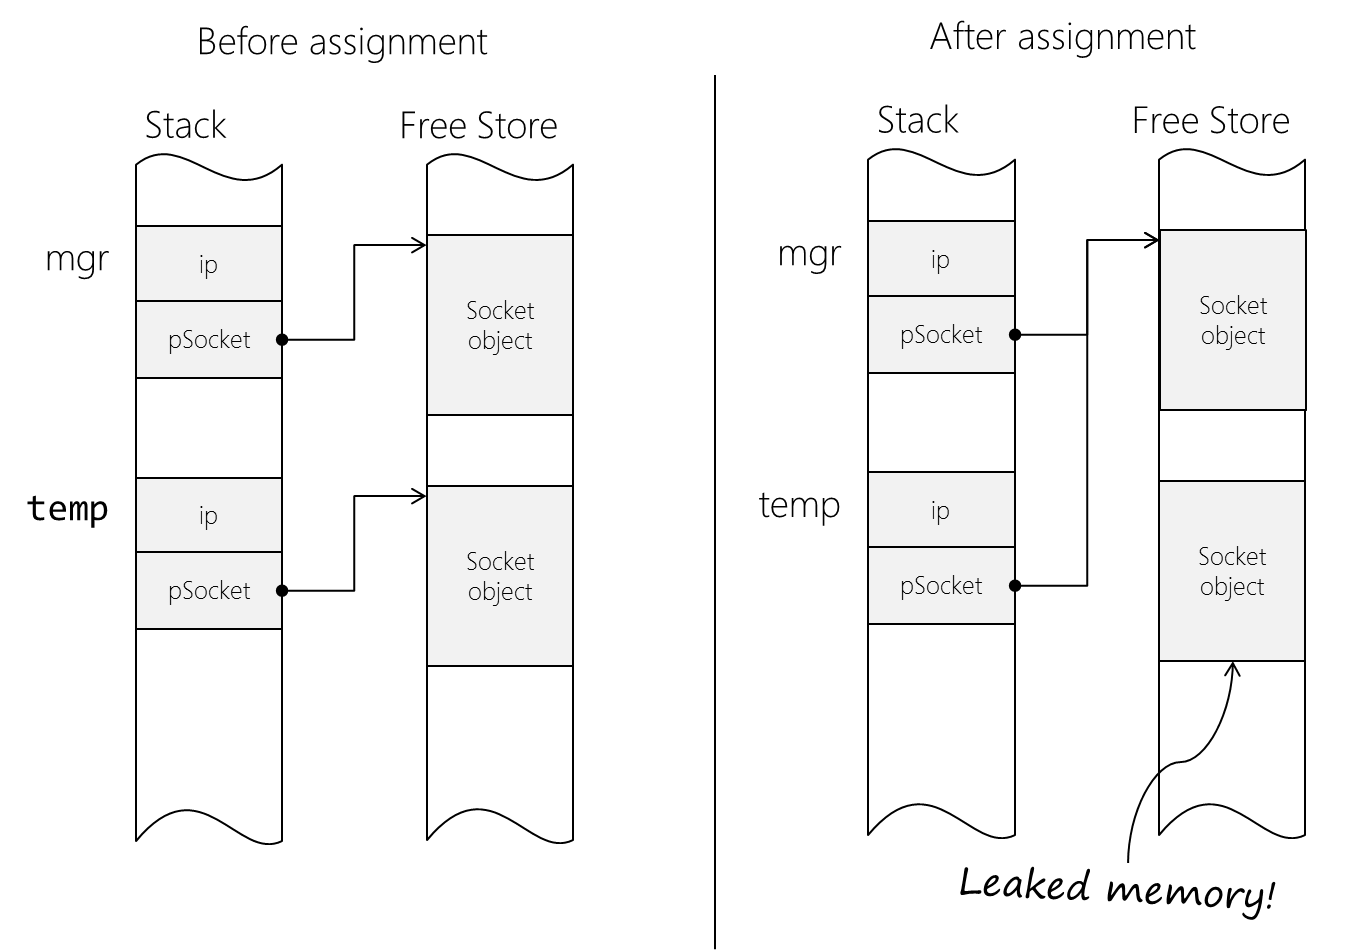
\includegraphics[width=14cm]{./imgs/image.644MS0.png}
\end{figure}

\indent{}通过上图给出的内存布局,我们可以很清楚地看到这其中潜在的另一危险之处。在\texttt{temp}刚被创建出来时,
其拥有自己所管理的\texttt{Socket}对象,\texttt{mgr}也管理着一个\texttt{Socket}对象。默认的赋值运算符会做
member-wise copy,那么在赋值之后,\texttt{temp}自己原本管理的那个\texttt{Socket}对象就失联了。
我们已经无法通过指针来对这个\texttt{Socket}对象的内存进行释放,所以这里存在内存泄漏。

\indent{}看来,编译器产生的默认赋值运算符在这里不能很好地完成工作。为了解决上述问题,我们需要自己提供赋值运算符
的实现。实现的要点是,在创建\texttt{temp}对象时创建出来的那个\texttt{Socket}对象是没什么用的,我们真正要用的还是
\texttt{mgr}所管理的\texttt{Socket}。并且,为了不让有用的\texttt{Socket}对象由于\texttt{temp}离开作用域而被销毁,
可以将这个有用的\texttt{Socket}对象拷贝一份,将其交给\texttt{temp}。

\begin{figure}[h]
\centering
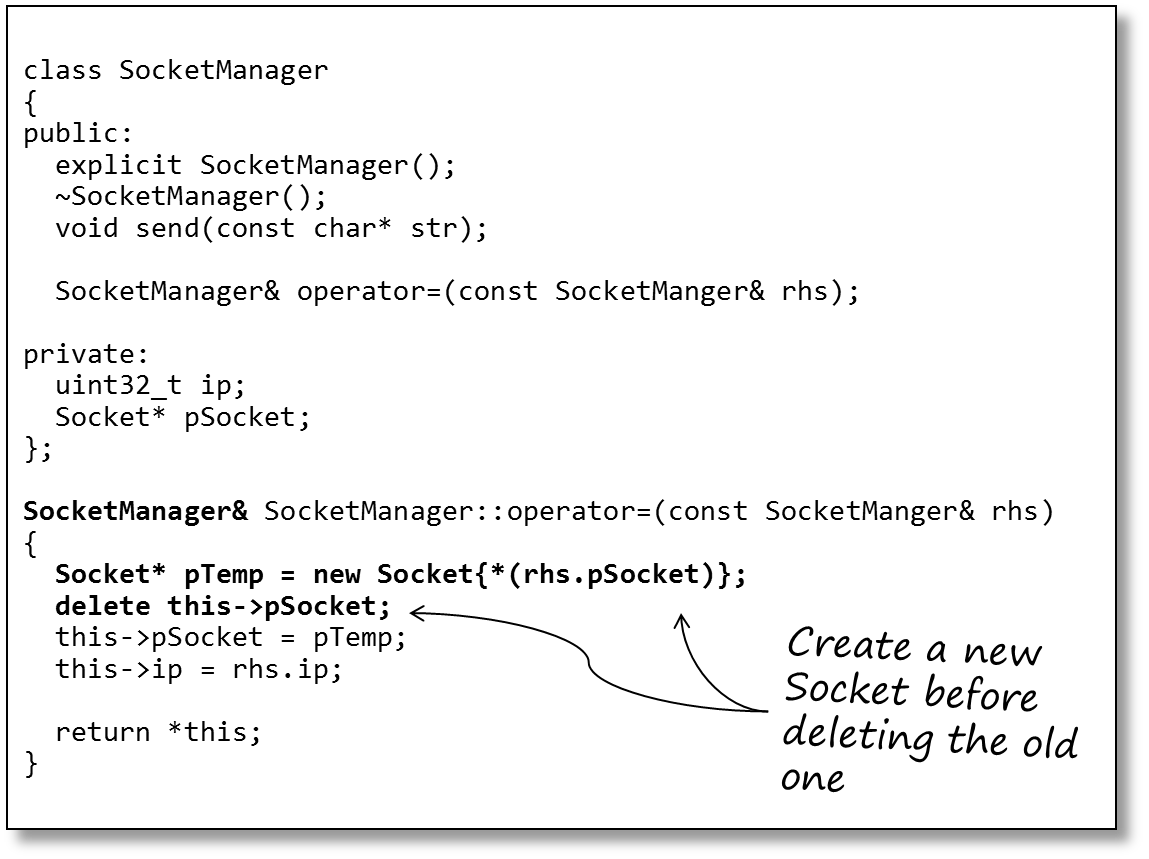
\includegraphics[width=10cm]{./imgs/image.C28HS0.png}
\end{figure}

\indent{}上述实现给出了执行深拷贝的赋值运算符,而不仅仅是将指针进行拷贝,它可以和 RAII/RRID在一起工作。
一个细节是这里实现的赋值运算符返回了被赋值对象的引用,用于支持串联的赋值操作。

\section{拷贝构造函数}
\indent{}如果我们没有为\texttt{SocketManager}类提供自己的拷贝构造函数,编译器就会提供一个做member-wise copy的
拷贝构造函数,这和之前我们讨论赋值运算符时遇到的情况相同。同样的,我们需要提供一个做深拷贝的拷贝构造函数,以
覆盖掉默认的拷贝构造函数。

\begin{figure}[h]
\centering
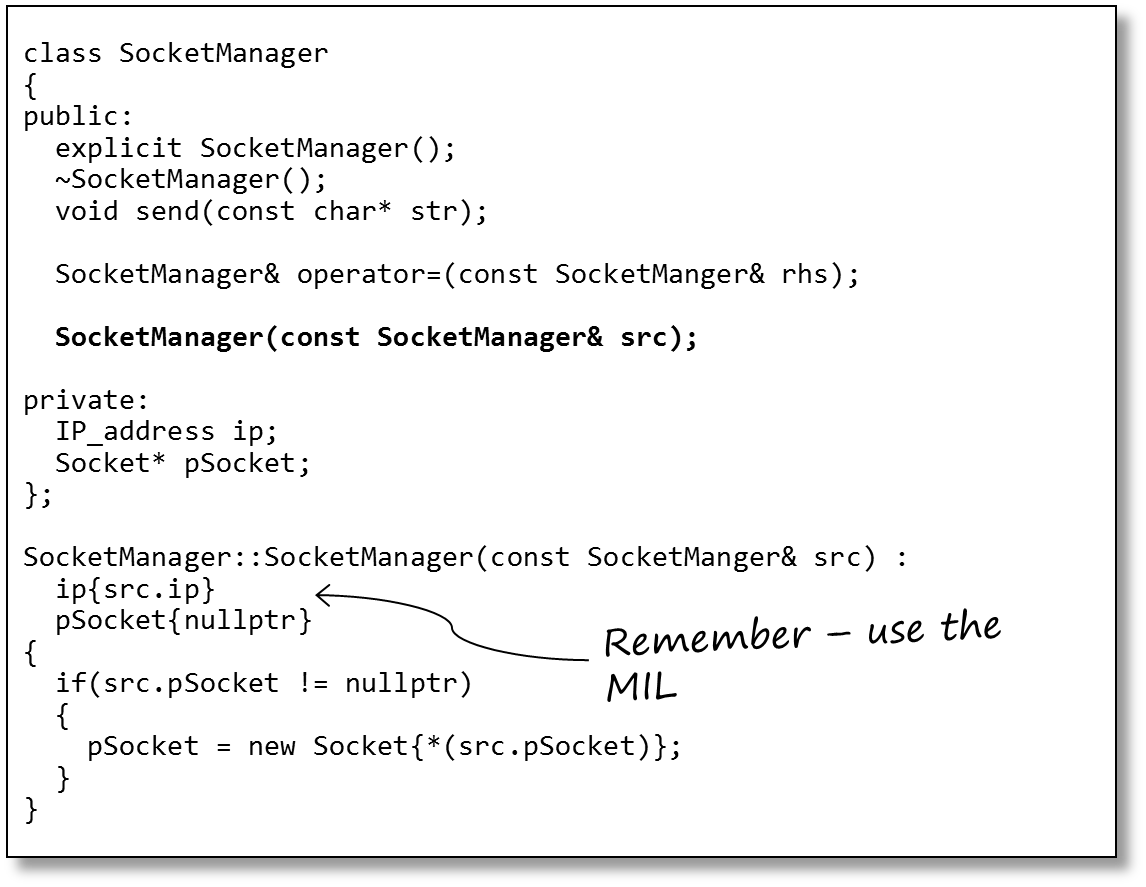
\includegraphics[width=11cm]{./imgs/image.QMRNS0.png}
\end{figure}

\indent{}拷贝构造函数以一个\texttt{const}的引用为参数,以其为样本来创建一个新的对象。注意到这里有一个实现细节,
我们检查传进来的对象是否真的管理着一个\texttt{Socket}对象,以免出现意料之外的结果。

\indent{}与赋值运算符不同,拷贝构造函数可能会在一些情形下被“隐式”地调用。
作为补充,让我们来思考一下拷贝构造函数会在何时被调用。可以总结出四种情况:
\begin{enumerate}
\item 显式拷贝构造:最直接的情况就是在显式地创建对象时调用拷贝构造函数。
\begin{figure}[!h]
\centering
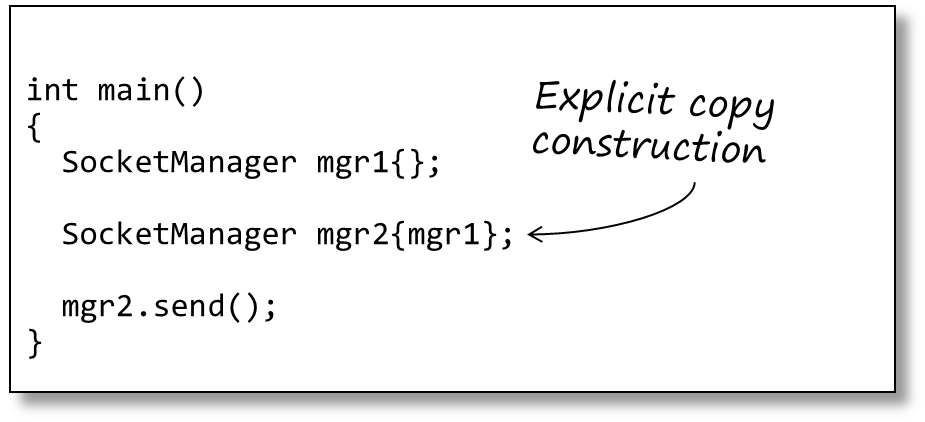
\includegraphics[width=7cm]{./imgs/image.UV9GS0.png}
\end{figure}
\item 对象的初始化过程:{\CC} 是区分初始化和赋值的。如果对象要被初始化,那么编译器会调用拷贝构造函数,而非赋值运算符。%
                        下述的例子展示了这一点。
\begin{figure}[!h]
\centering
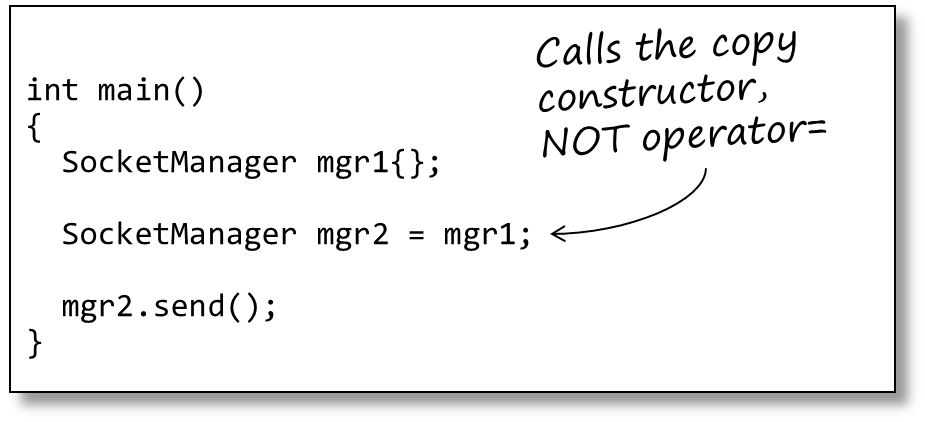
\includegraphics[width=7cm]{./imgs/image.X51GS0.png}
\end{figure}
\item 以传值(Pass-by-value)的方式传参:如果对象被以传值的方式传给函数,那么会创建一份拷贝。
\begin{figure}[!h]
\centering
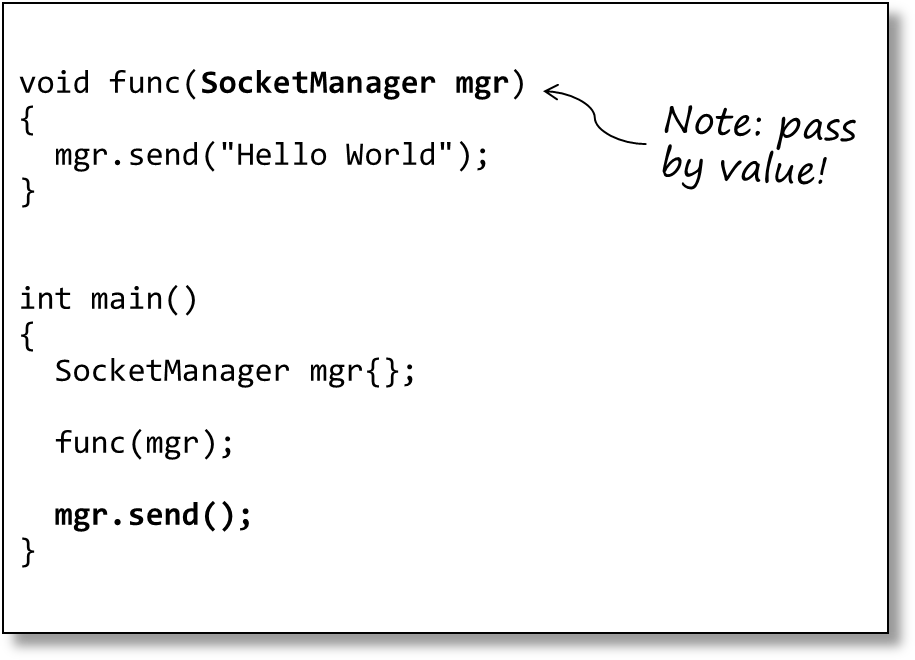
\includegraphics[width=7cm]{./imgs/image.ANABS0.png}
\end{figure}
\item 函数的返回值:如果一个函数以值的形式返回一个对象,那么会创建一份拷贝。
\begin{figure}[!h]
\centering
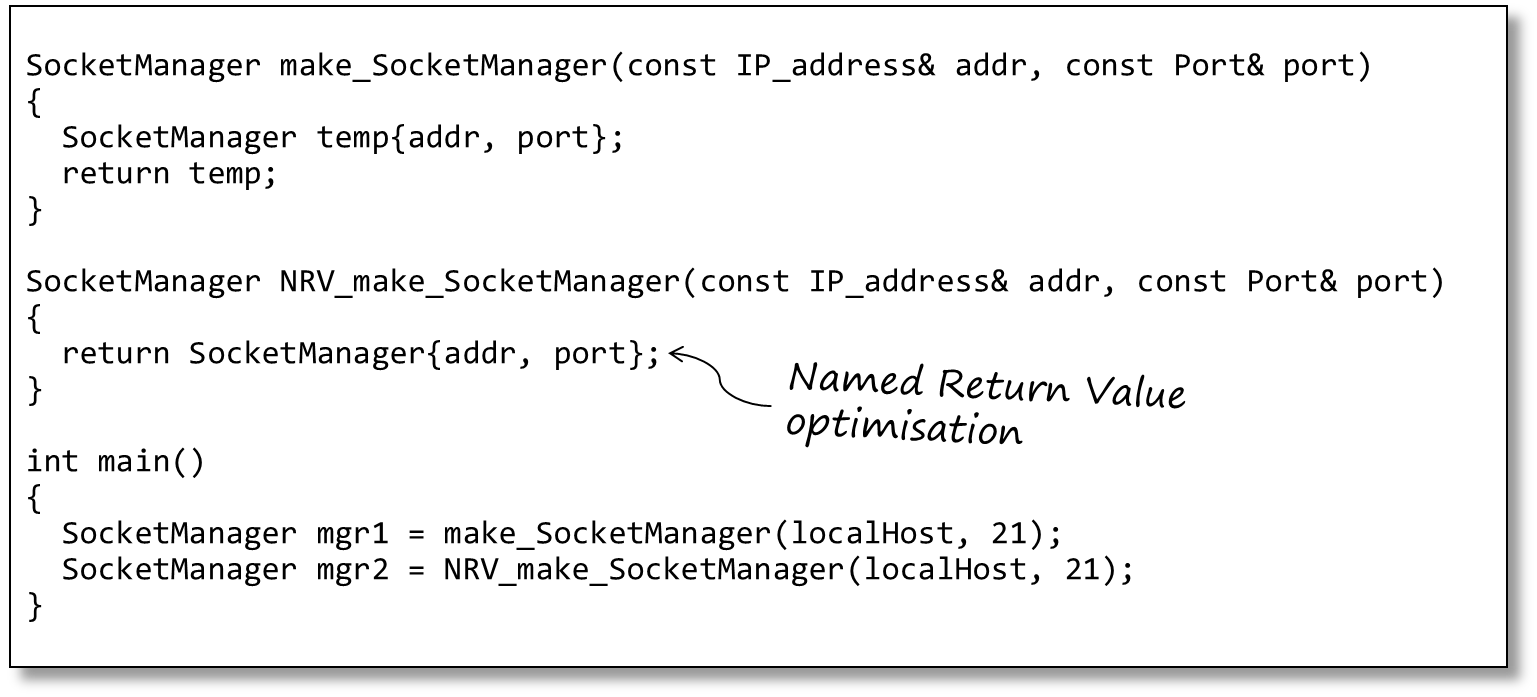
\includegraphics[width=10.2cm]{./imgs/image.TX9KS0.png}
\end{figure}
\end{enumerate}

\indent{}第四种情况比较特殊,因为这里可以进行NRV(Named Return Value)优化。如果返回的对象直接作为返回语句的
一部分被构造,编译器可能会针对这种情形进行优化,将要返回的对象直接构造到 caller object。在这种情形下,normal的
构造函数会被调用,而不是拷贝构造函数。

\section{移动构造函数}
\indent{}在很多情况下,拷贝一个对象并不是最好的选择。因为这可能是开销很高的,涉及到临时对象的创建,拷贝和析构
过程。比如下面的一些情形:
\begin{enumerate}
    \item 从函数返回对象
    \item 一些算法的实现(比如\texttt{swap})
    \item 容器的动态分配
\end{enumerate}
\noindent{}我们以\texttt{SocketManager}的\texttt{vector}为例进行说明:
\begin{figure}[h]
\centering
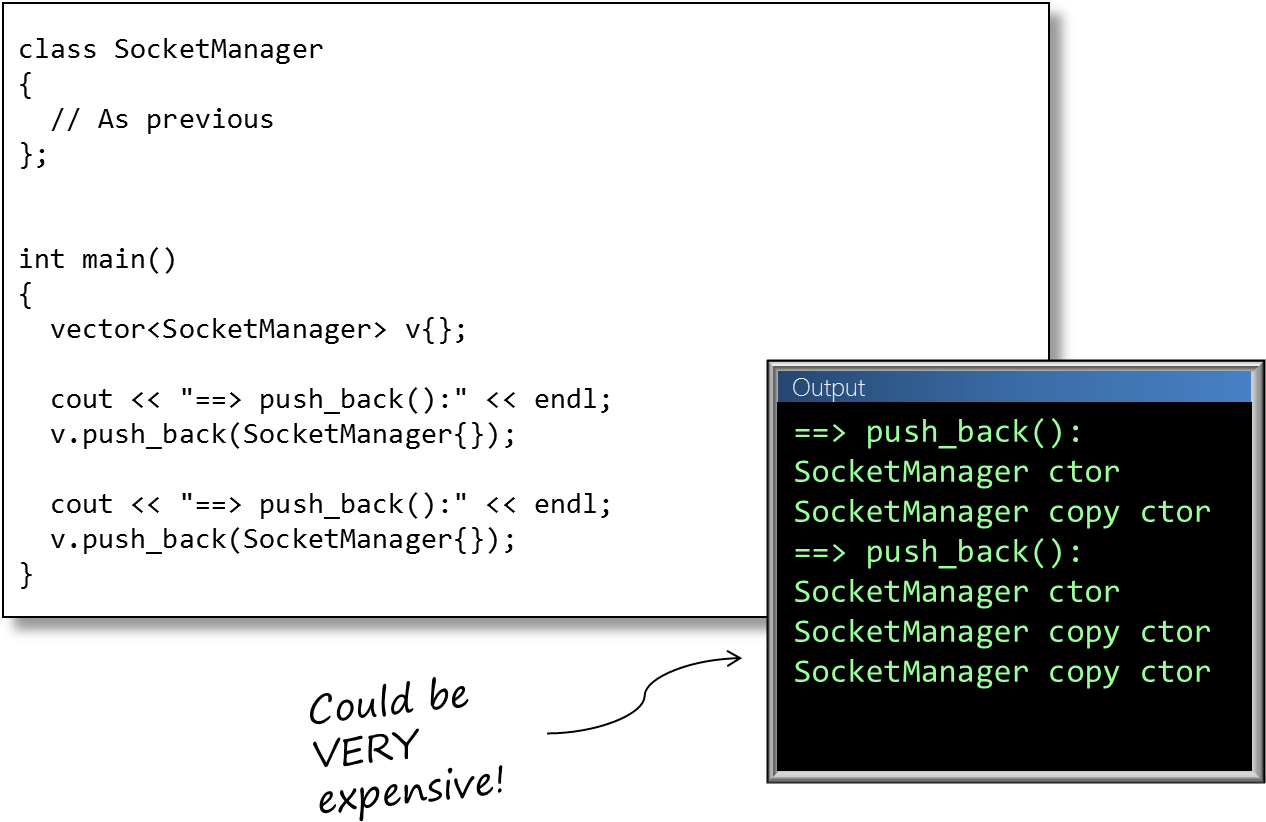
\includegraphics[width=10cm]{./imgs/image.MP3AS0.png}
\end{figure}

\indent{}可以看到,第二次的\texttt{push\_back}伴随着两次拷贝构造函数。之所有会有第二个拷贝构造过程,是因为
\texttt{vector}的内存分配器会先分配两个\texttt{SocketManager}对象所需的空间,然后将两个对象分别拷贝过来。
这是一个开销很大的过程,因为每次都会伴随着内存的de-allocation与re-allocation,还要拷贝对象相应的内容。
实际上,我们通常只想将数据从一个对象transfer到另一个对象。

\indent{}{\CC}98中,经常会有开销高昂的拷贝。当临时对象被创建时,他们就将要被拷贝。许多情形下,这种拷贝是很不必要的,
因为临时对象马上就会被丢弃。

\begin{figure}[!h]
\centering
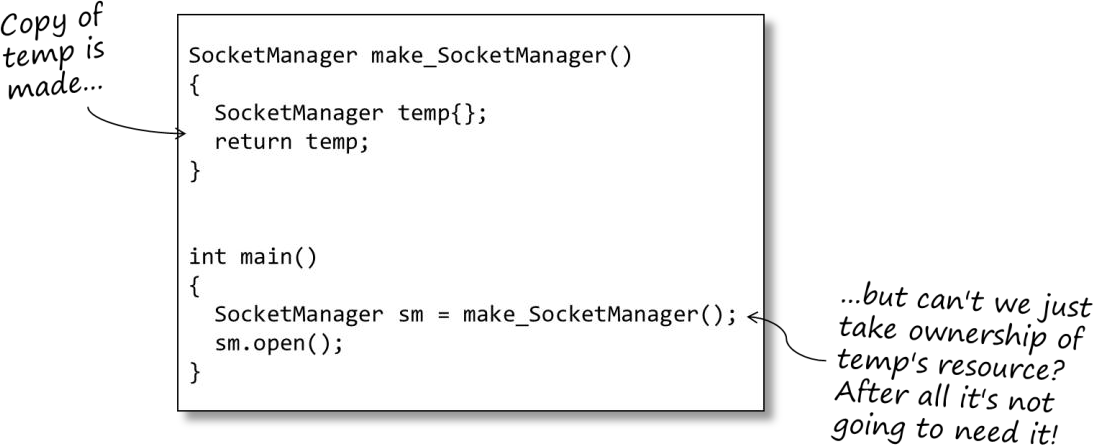
\includegraphics[width=11cm]{./imgs/image.FNFHS0.png}
\end{figure}

\indent{}如果我们可以只是拿到临时对象的资源的“所有权”就好了,这可以让我们从de-allocation与re-allocation
的重担中解放出来。这种拿到“所有权”的手段有时也被称为“资源窃取”。我们需要做的是以某种方式区分临时对象(他们马上
就要离开作用域)与在语句之后会继续存在的对象。

\indent{}让我们先来谈谈右值(r-value)吧。我们知道,左值(l-value)的原意是可以被放在赋值运算符左侧的表达式。
与之对应的,右值的原意正相反,是指不可以被放在赋值运算符左侧,只能被放在赋值运算符右侧的表达式。{\CC}11 添加了
一些更为细微的的术语,进而复杂化了上述定义。从便于理解的角度来看,我们可以先专注于{\CC}03 中的含义。如果我们
有:

\begin{minted}[mathescape=true,
               linenos,
               numbersep=5pt,
               autogobble,
               frame=lines,
               fontsize=\small,
               bgcolor=bg,
               framesep=2mm]{C++}
    int x;
\end{minted}

\indent{}我们给\texttt{x}赋值是没什么问题的,比如\texttt{x = 42}。所以\texttt{x}是一个左值表达式。
作为其反例,如果我们写\texttt{x + 0 = 42}显然是不行的,因而\texttt{x + 0}是一个右值表达式。类似的,
\texttt{2 + 2}也是右值表达式。

\indent{}一个引用类型的表达式必须指向一个具有明确内存地址的对象(即表达式是左值)。然而,除了引用性外,类型
和rvalue/lvalue之间并无关联。比如说,\texttt{x}和\texttt{x + 0}都是类型为\texttt{int}的表达式,而且他们给出
相同的整型的值。但是前一个表达式是左值表达式,后一个表达式是右值表达式。

\indent{}我们可以用一个简单的方法来判断左值与右值:左值是指向确切内存位置的,而右值不指向任何地方。一般来说,
右值是临时的,生命期很短的,左值是以变量形式存在的,具有较长生命期的。一个很形象的比喻是,可以将左值看成是
放东西的盒子,而右值是盒子里放的东西。如果你可以将built-in的取地址运算符作用上去,那么它就是左值表达式。
否则,就是右值表达式。

\indent{}{\CC}11 引入了右值引用,一个右值引用可以被显式地绑在一个右值上。右值引用本身虽然不是特别有用,但它
可以和函数重载技术搭配使用,用于与左值引用区分,针对传入的rvalue类型的参数进行响应,以给出相应的行为。

\begin{figure}[h]
\centering
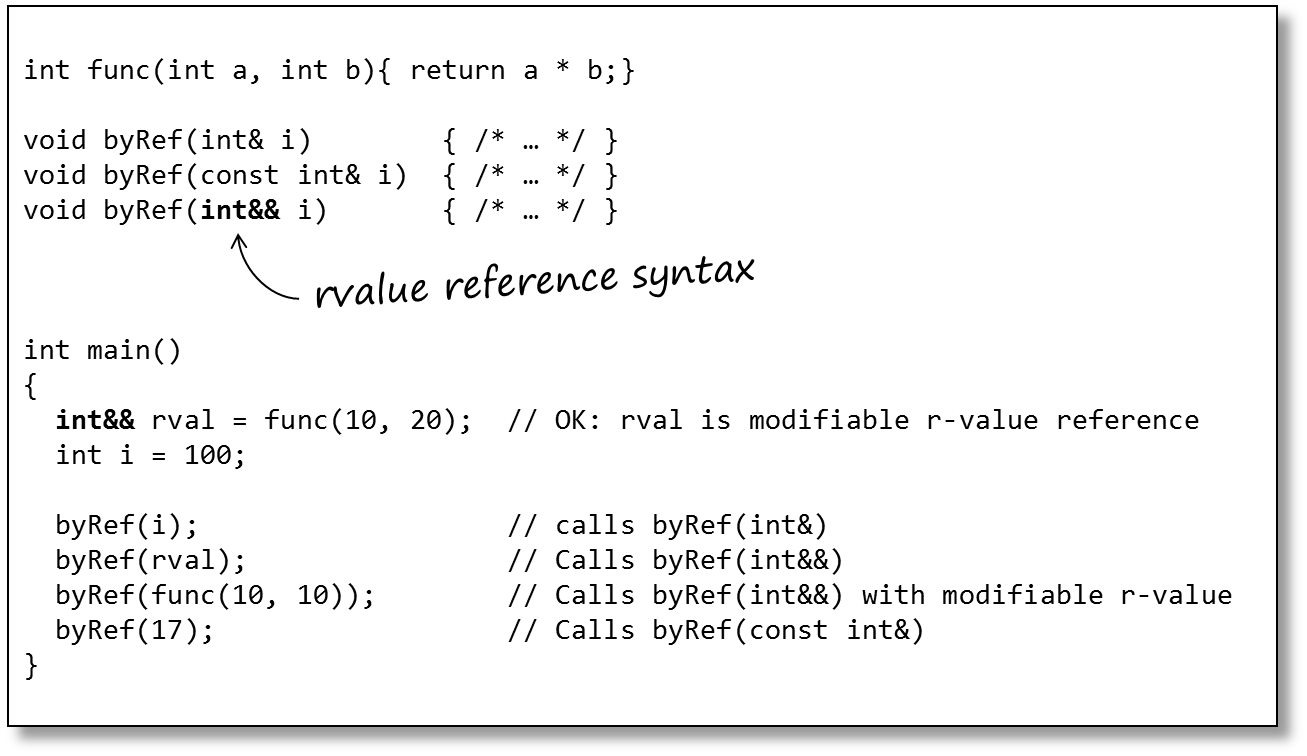
\includegraphics[width=12cm]{./imgs/image.F3BZS0.png}
\end{figure}

\noindent{}对于右值引用,仅匹配到可被修改的右值。对于常量右值,会匹配到\texttt{const}的左值引用上。

\indent{}既然我们已经可以区分左值与右值对象,那么我们可以重载构造函数(相同的,还有后面将要提到的赋值运算符)
来支持资源窃取。即实现移动构造函数:

\begin{enumerate}
    \item 以右值引用为参数
    \item 丢弃对象的当前状态
    \item 将右值对象的所有权转移至接受方
    \item 将右值对象置为“空”状态
\end{enumerate}

\begin{figure}[h]
\centering
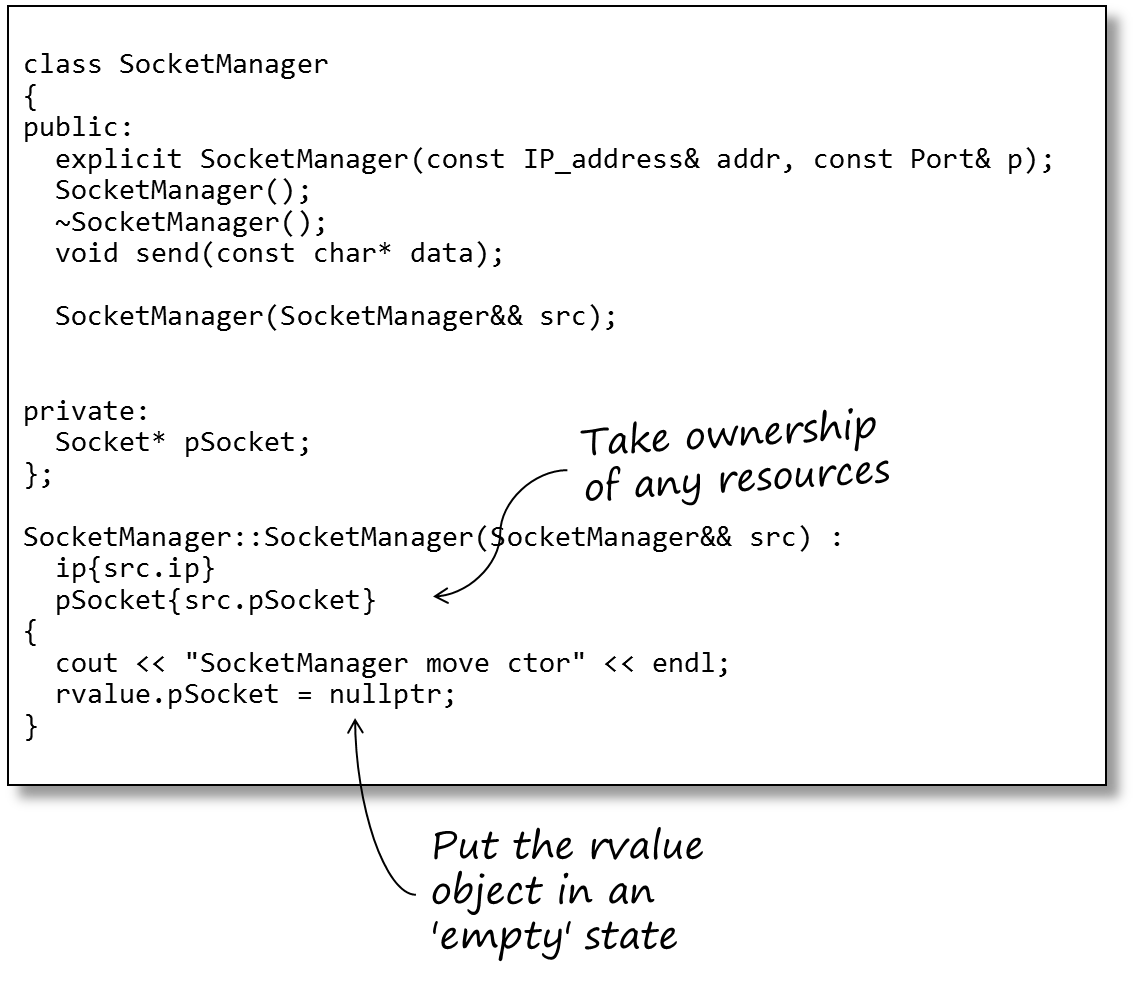
\includegraphics[width=12cm]{./imgs/image.K672S0.png}
\end{figure}

\noindent{}注意移动构造函数的参数不是\texttt{const}的,因为我们需要改变参数本身。

\indent{}移动构造函数对提供的右值的资源进行宣称。由于右值的\texttt{pSocket}被置为\texttt{nullptr},则
在右值离开作用域时,其析构函数不会做任何事情。

\begin{figure}[h]
\centering
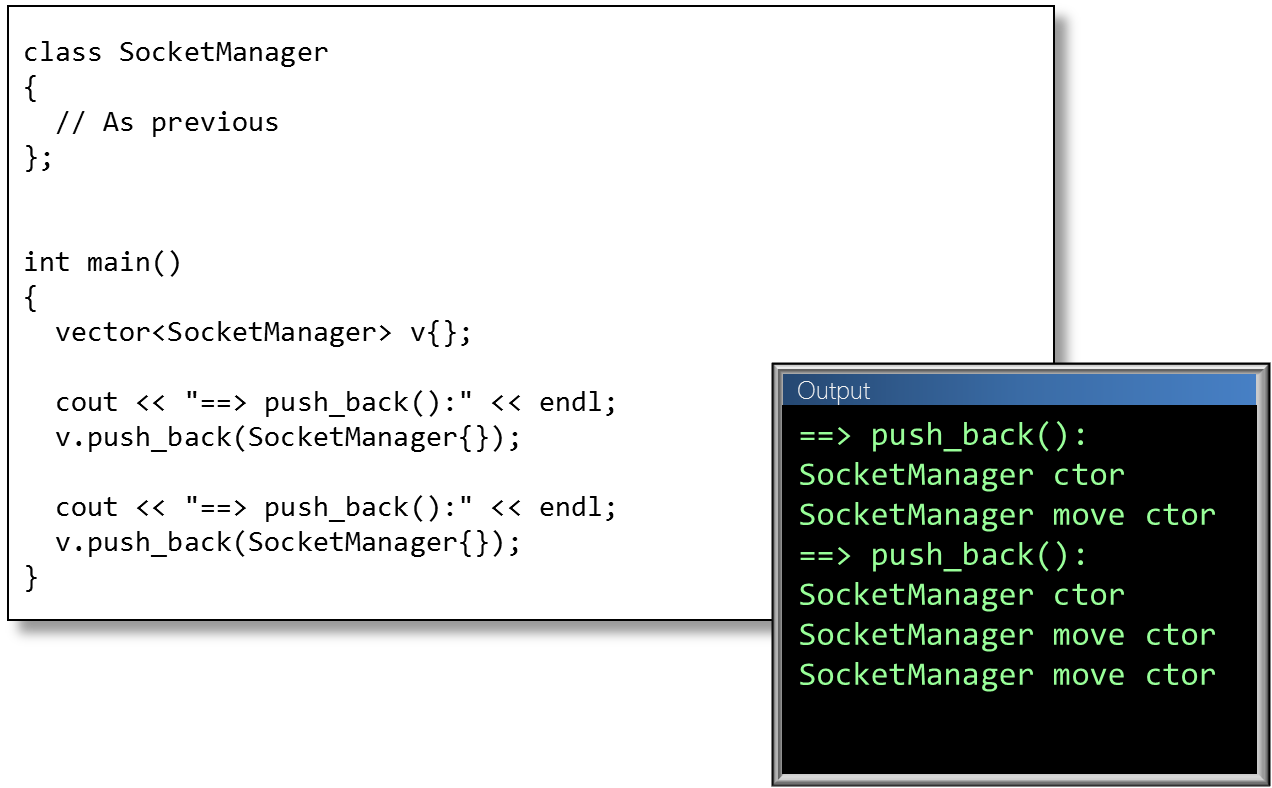
\includegraphics[width=11cm]{./imgs/image.ZZAZS0.png}
\end{figure}

\indent{}回到我们的有关\texttt{SocketManager}的\texttt{vector}的问题。因为现在\texttt{SocketManager}有了
移动构造函数,所以不会有临时对象的拷贝发生。这样的代码更为高效。

\indent{}这里补充一点,如果你想要在派生类中包含move语义,需要仔细处理。如果你希望从派生类中应用基类的移动语义,
你必须显式地使用\texttt{std::move}将左值转换为右值,才能匹配到基类的移动构造函数。否则的话,还是会调到基类的拷贝构造函数。

\begin{figure}[h]
\centering
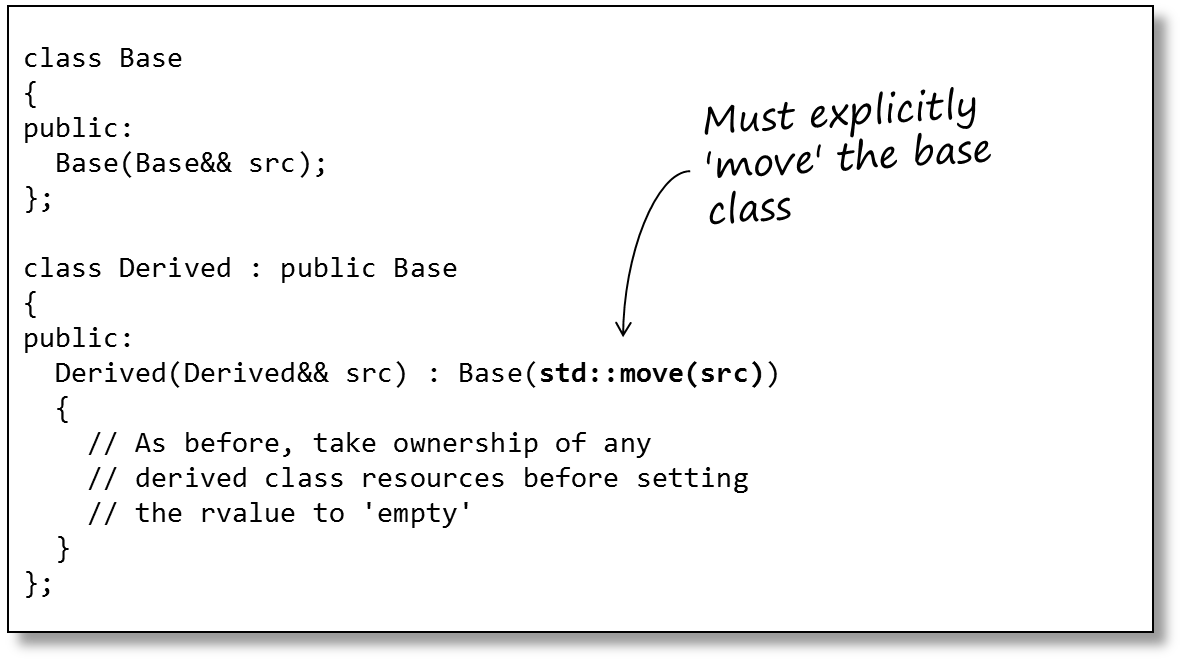
\includegraphics[width=10cm]{./imgs/image.QXK6S0.png}
\end{figure}
\noindent{}上图给出了这个要点的一个例子。

\section{移动赋值运算符}
\indent{}有时,我们希望在同一时刻只保留一份某资源,并且我们能够将这一份资源的所有权从一个管理者转移到
另一个管理者那里(就像\texttt{std::unique\_ptr}所做的那样)。在这种情况下,我们需要提供移动赋值运算符
来支持这种资源的所有权转移。

\begin{figure}[h]
\centering
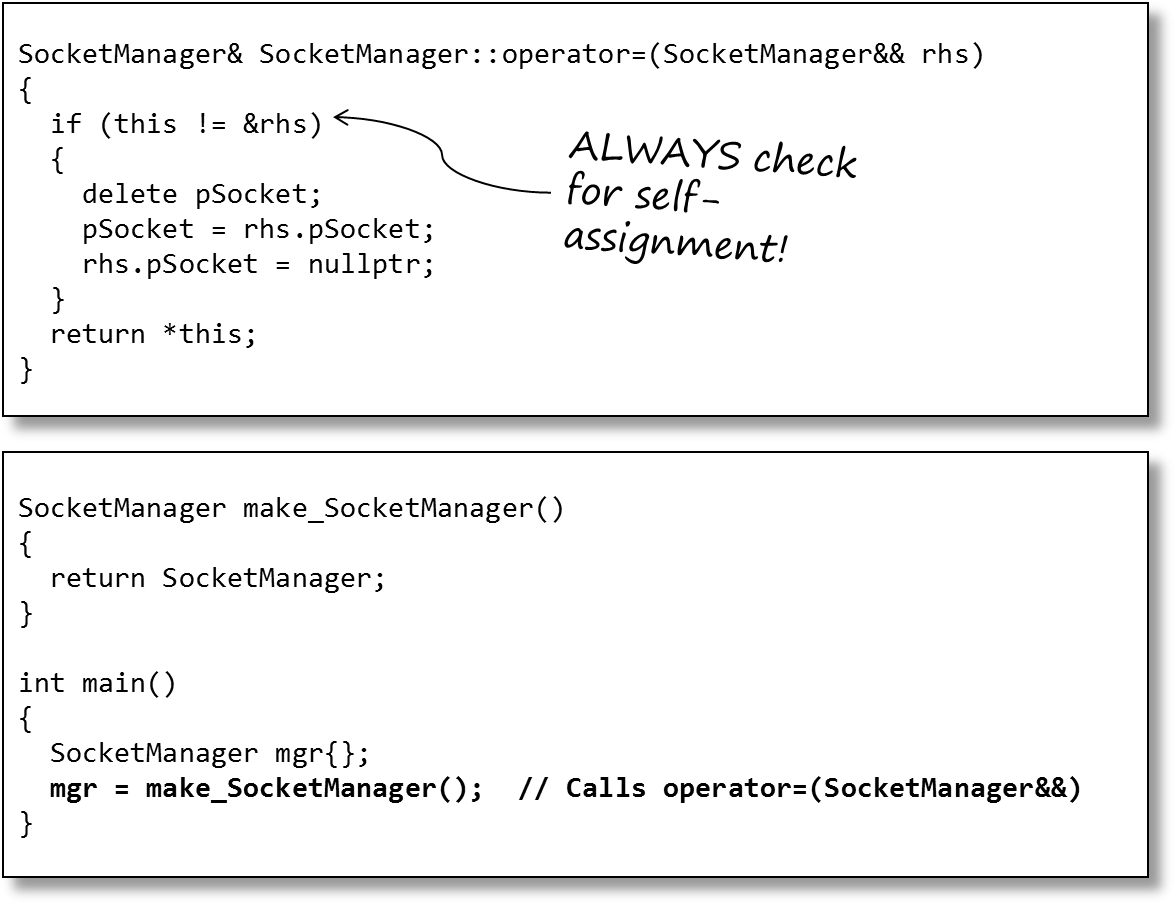
\includegraphics[width=10cm]{./imgs/image.F07TS0.png}
\end{figure}

\indent{}需要注意的是,我们总是需要检查自赋值的情况。尽管这在手写的代码里很罕见,但是在
一些算法的运行中这确实有可能发生(例如\texttt{std::sort})。另外,注意将上述代码
中\texttt{mgr = make\_SocketManager()}与对象的初始化过程区分开。在这个例子里,\texttt{mgr}已经被初始化过了,
所以这里执行的是赋值操作。

\section*{资源管理策略}
\indent{}五之法则说明,如果你已经写出了上述五个函数中的一个,那么你必须对其他的函数有相应的策略。
这并不是在说你必须要写出他们。实际上是,你必须为你的每个类提供资源管理策略。下列给出了一些可能的资源管理策略:

\begin{itemize}
    \item 使用编译器提供的这些函数的版本(实际上只有前三个,编译器不会自动提供后两个移动函数)
    \item 写出自己的拷贝函数来做深拷贝,不使用move semantic
    \item 写出自己的移动函数,不提供拷贝
    \item 禁止拷贝和移动,因为允许这些操作并无意义(对于有些类确实是这样)
\end{itemize}

\noindent{}禁止拷贝和移动是很容易实现的,主要有两种方式:
\begin{itemize}
    \item 把相应的函数声明放在\texttt{private}下({\CC}98 的手法)
    \item 使用\texttt{=delete}记法({\CC}11 的手法)
\end{itemize}
\begin{figure}[h]
\centering
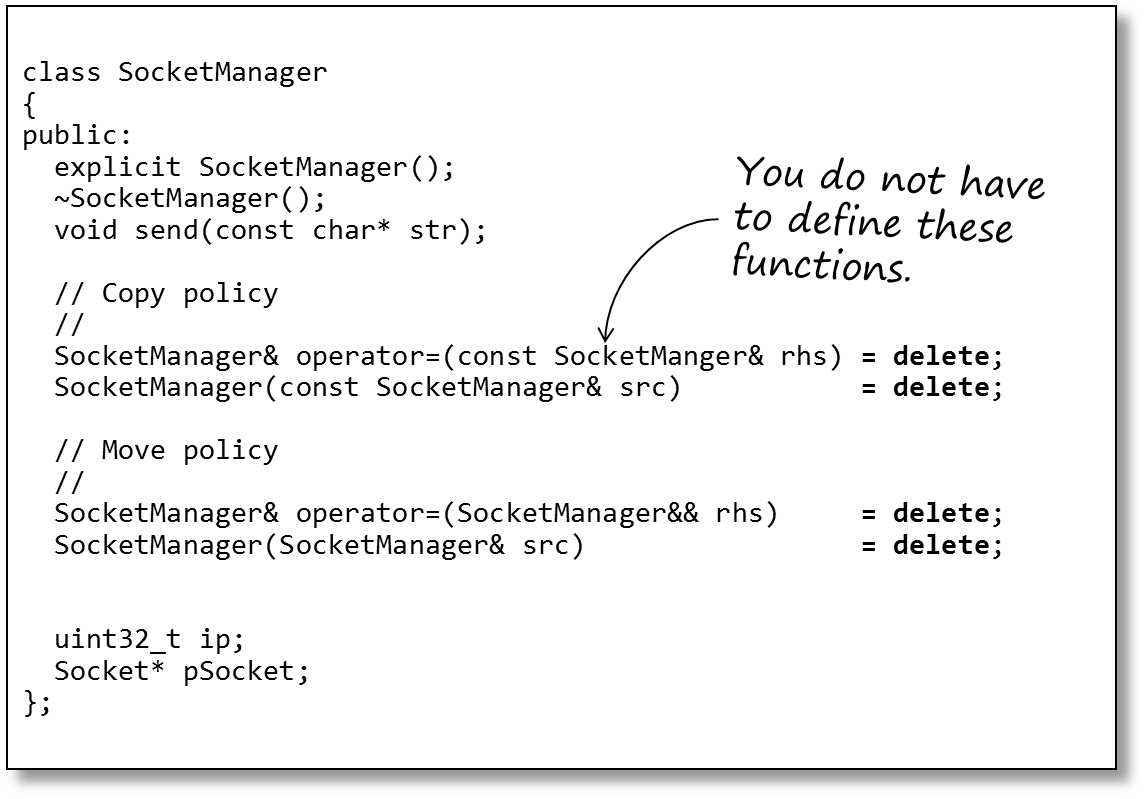
\includegraphics[width=12cm]{./imgs/image.BBM0S0.png}
\end{figure}

\section*{结论}
\indent{}资源管理,即使用{\CC} 的RAII/RRID 机制,是构建高效可维护且bug-free代码的关键。为系统中的每个类定义
你的拷贝和移动策略是软件设计的关键部分。五之法则是你的copy/move策略的备忘录。你可以放轻松去忽略它,但这也会
带来危险。最后要说的是,审视移动和拷贝策略也会促成两点作为补充的很好的实践:
\begin{itemize}
    \item 一个类应该只管理最多一个资源
    \item 使用现有的资源管理类(比如智能指针)来简化你的类的设计
\end{itemize}

\end{document}